\documentclass[12pt, a4 paper]{article}
\usepackage[british]{babel}
\usepackage{graphicx, hyperref, xcolor, fancyhdr, amssymb, amsmath, amsthm, mdframed, tikz}
\usepackage{mathrsfs}
\usepackage[acronym, toc]{glossaries}
\usepackage{pdfpages}
\usepackage{svg}
\usepackage{algorithmic}
\usepackage[ruled, linesnumbered]{algorithm2e}


% editorial comments in the text or in marginal notes
% 1st argument: initials of the person making the comment,
% 2nd argument: comment to insert
\long\def\ednote#1#2{\par\noindent\framebox{\begin{minipage}{.98\linewidth}\linespread{.7}\footnotesize #1: #2\end{minipage}}\par}
\newcommand{\edmargin}[2]{\marginpar{\raggedright\linespread{.7}\tiny #1: #2}}

% redefine proof environment with grey background and black square at the end
\renewenvironment{proof}[1][Proof]{\begin{mdframed}[backgroundcolor=black!5, topline=false, rightline=false, bottomline=false, linecolor=black!15, linewidth=3pt]{\noindent\textit{#1.}\ }}{\noindent\par\hfill$\blacksquare$\end{mdframed}}

% \usepackage{times}

\hypersetup{
    colorlinks,
    linkcolor={red!60!black},
    citecolor={blue!80!black},
    urlcolor={blue!80!black}
}

% \pagestyle{fancy}
% \renewcommand\headrulewidth{.5pt}
% \fancyhead[L]{
%     V. Trélat
% }

% \fancyhead[C]{
%     \textbf{Verification in Isabelle/HOL of Hopcroft's algorithm for minimizing DFAs including runtime analysis}
% }

% \fancyhead[R]{
%     % Current section
%     \ifnum\c@secnumdepth>0
%         \thesection
% }

% theorems
\theoremstyle{definition}
\newtheorem{theorem}{Theorem}
\newtheorem{lemma}{Lemma}
\newtheorem{remark}{Remark}
\newtheorem{definition}{Definition}
\newtheorem{requirement}{Requirement}

% Glossary

\makeglossaries

% \newacronym{tiaa}{TIAA}{This Is An Acronym}

\begin{document}

\begin{titlepage}
    \begin{center}
        \vfill
        
\includegraphics[height=1.5cm]{img/logoTUM.png}
        \hfill
        
\includegraphics[height=1.5cm]{img/logoartem.png}
        \hfill
        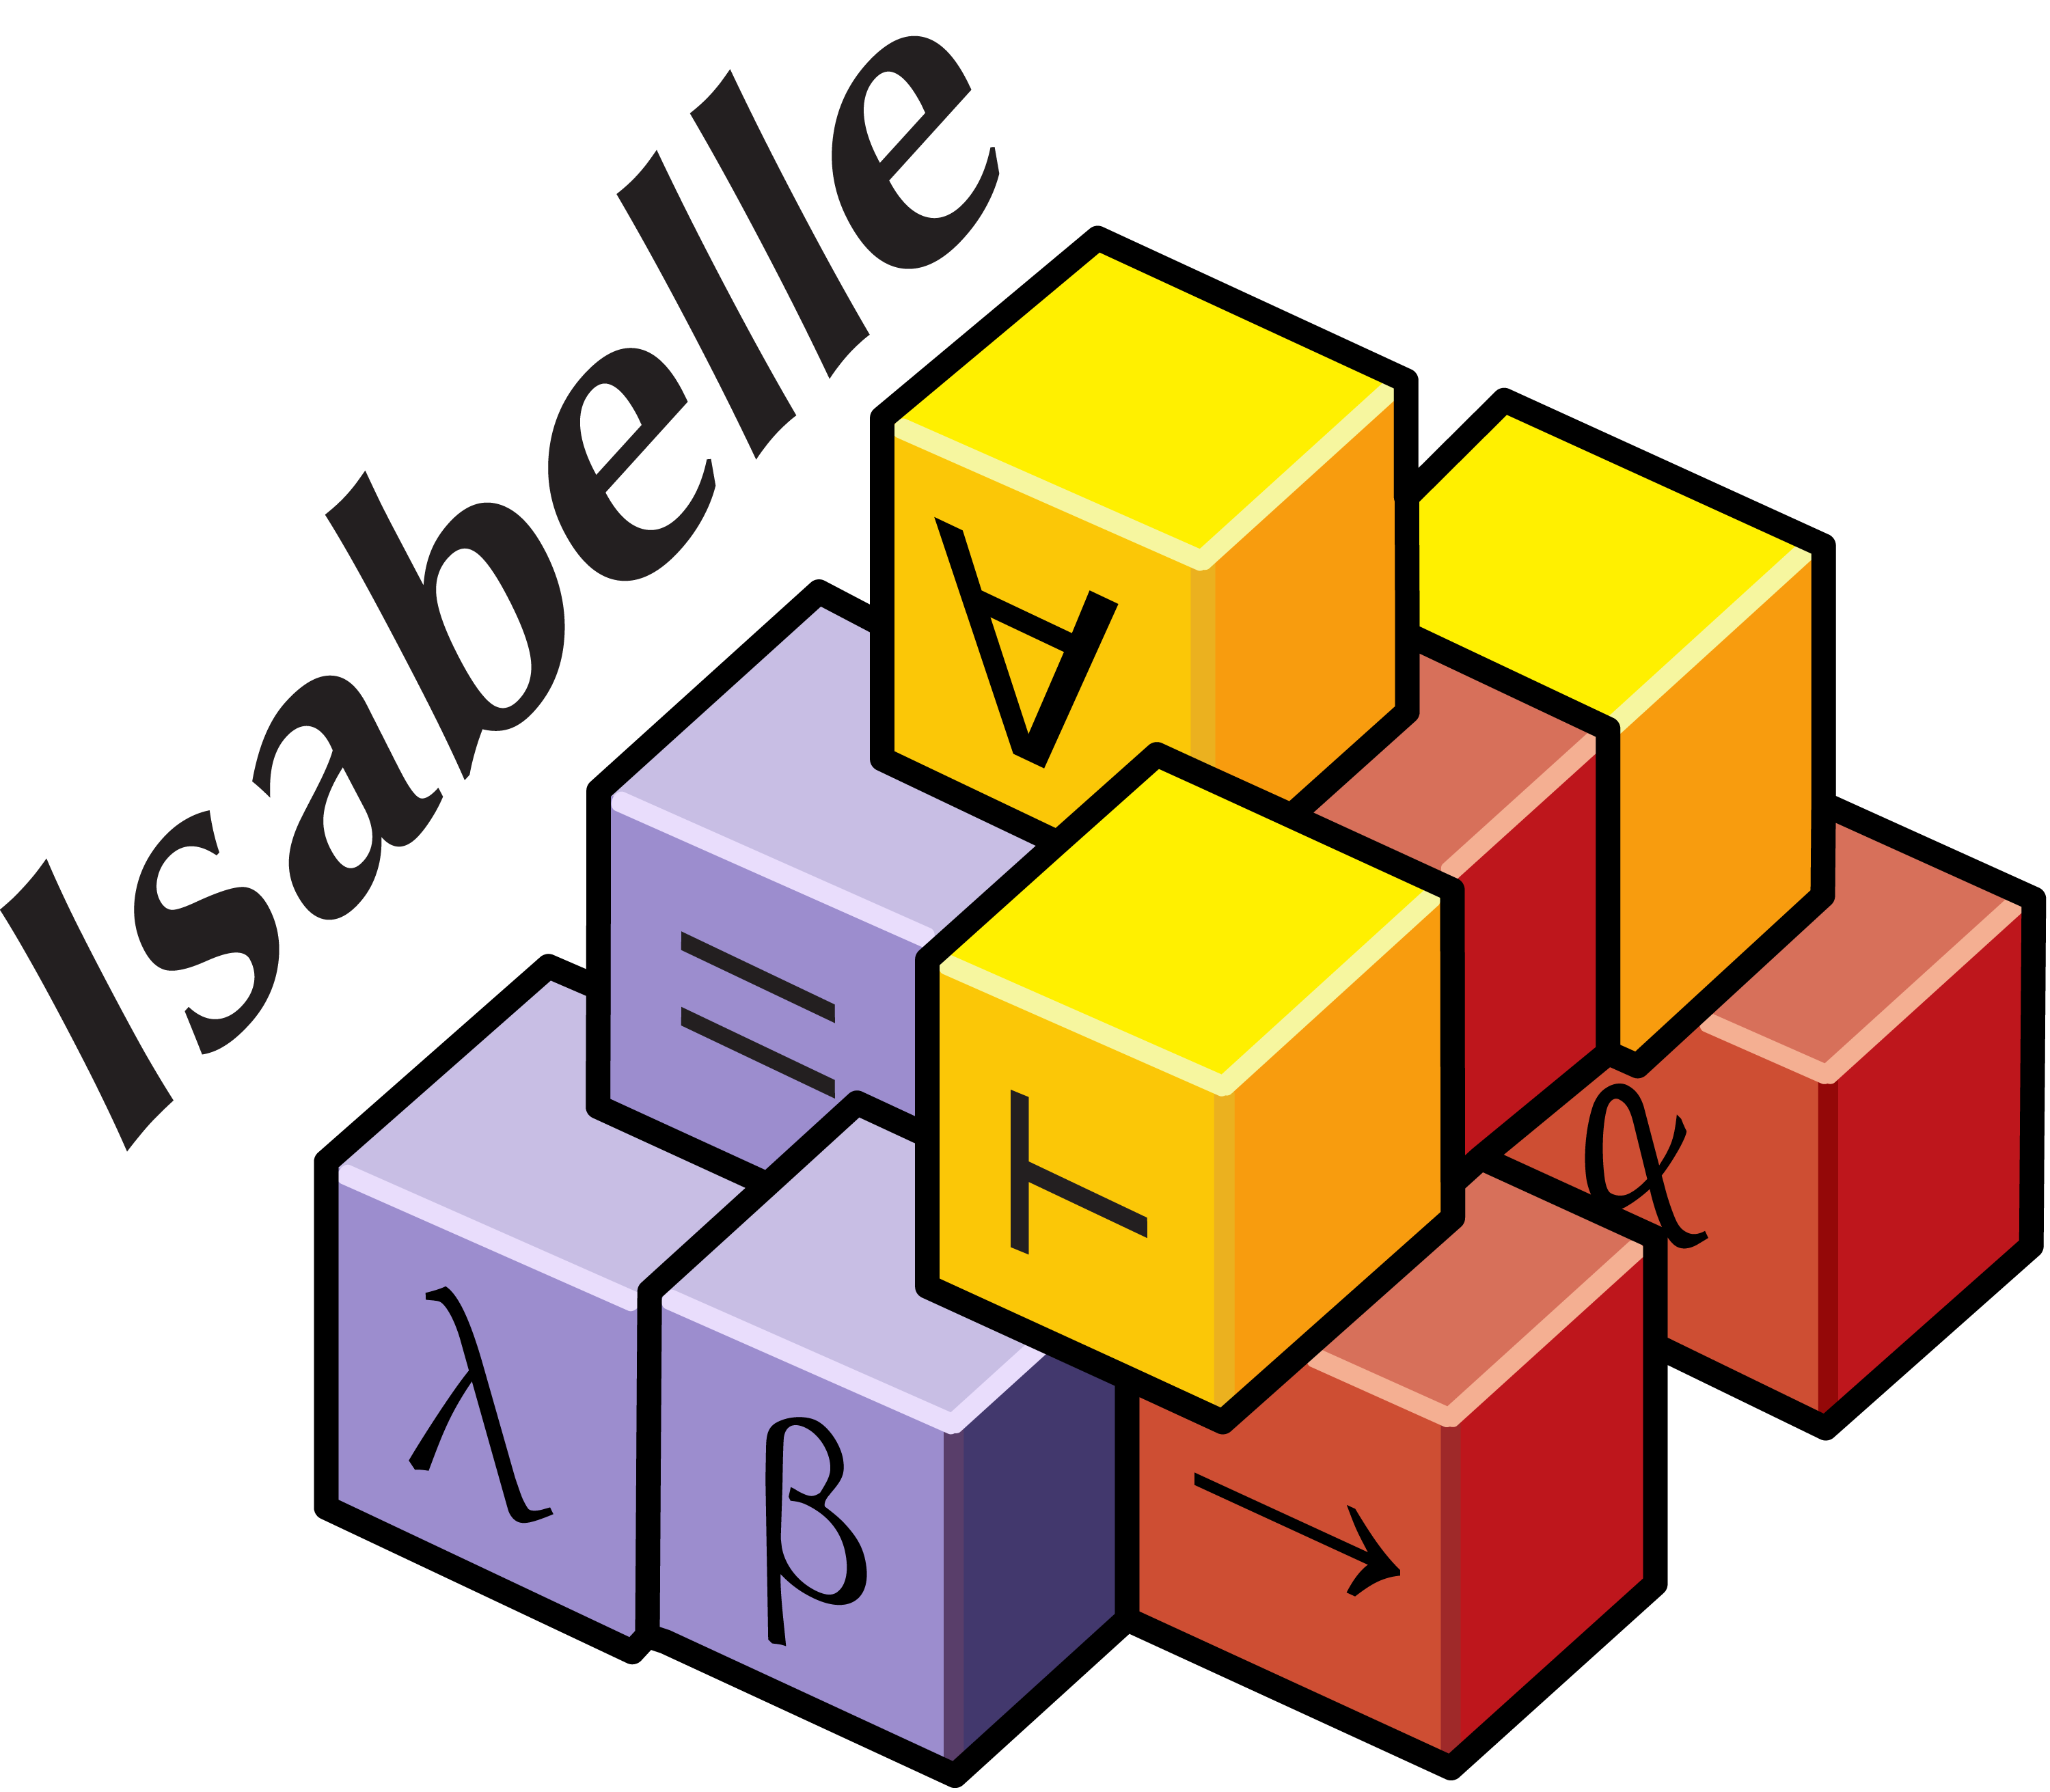
\includegraphics[height=1.5cm]{img/logoisabelle.png}
        \vfill
    \end{center}
    \begin{center}
        
        \textbf{Final year internship report}
        \vfill

        \large{\textbf{Verification in Isabelle/HOL of Hopcroft's algorithm for minimizing DFAs including runtime analysis}}
    \end{center}
    
    \vfill
    
    \begin{center}
        \textbf{Vincent Trélat}\\
        \vspace{1cm}
        \textit{\today}
    \end{center}
    \vfill
    \begin{center}
        
\includegraphics[height=1.2cm]{img/logoGE.png}
        \hfill
        
\includegraphics[height=1.2cm]{img/logoUL.png}
    \end{center}
\end{titlepage}

\tableofcontents

\pagebreak

\section{Preamble}

Since the whole project relies on many deeply theoretical notions such as abstraction, logic or semantics, this section only gives a brief introduction to formal methods in general and their purpose.

\bigskip

Formal methods refer to a field of theoretical computer science whose main purpose is to provide logical links between mathematics and programming languages, so that one can state logical properties about formally described algorithms or mathematical procedures and relate them to actual implementations. The main application of formal methods is to prove correctness of programs with respect to a specification, i.e.\ a set of rules which must hold throughout the execution of the program. Such a program is then ensured to behave in a way\footnote{In the context of industrial applications, we often differentiate between two sorts of assertions, namely safety properties and liveness properties, so that we can explicitly check that the system works (it is ``alive'') and that it is safe (it works properly).} that is intended by its specification.

Such work is usually carried out using a proving assistant such as \href{https://isabelle.in.tum.de}{Isabelle}, i.e.\ a program with an implemented logic allowing to reason with respect to that logic. Isabelle has the advantage to relie on a really light kernel, which is the only part that can only be trusted. Everything else -- i.e. librairies, called theories -- stems from this kernel. It also has nice interface with \LaTeX syntax adding little overhead to usual mathematical notations and is very flexible in terms of syntax and semantics.

A common way to proceed when we want to prove correctness of an algorithm and generate correct executable code is to follow a top-down strategy via successive refinements. We start from the highest level -- i.e.\ with the highest level of abstraction -- and we refine towards the implementation. As an example, if an algorithm manipulates sets at the abstract level, we may use lists or trees in its implementation. When performing a refinement, we have to give links -- and prove them -- between levels, e.g. that the behavior of the refined one does not contradict the abstract one. In Peter Lammich's Refinement Framework \cite{lammich:ref}, this is done via binary relations and abstraction/concretization functions\footnote{A concretization function maps an abstract value to a set of concrete values and conversely for an abstraction function, so that invariants can be carried and preserved through the refinements. For example, we may abstract the set $\mathbb{Z}$ of integers to $\{Neg, Zero, Pos\}$ where $Pos$ (resp.\ $Neg$) represents positive (resp.\ negative) integers and $Zero$ represents the singular set $\{0\}$.}.

\bigskip

If formal methods allow for correctness and termination theorems, it is less trivial to analyze complexity of a program, e.g.\ in terms of time or memory consumption. Since complexity of a program is not a logical property, but a property of the execution of the program, a model of computation must be defined, i.e.\ a way to execute the program, and then prove that the execution of the program in this model is equivalent to the execution of the program in the real world. Maximilian Haslbeck and Peter Lammich have extended the Refinement Framework to include worst-case time complexity analysis in Isabelle \cite{refwithtime} and have also implemented a verified framework to analyze algorithms down to LLVM code \cite{fewdollarsmore}. The principle is to model costs of operations with resources and currencies and embed this new dimension in the program, where operations consume resources.

\bigskip

Since the project also relies on automata theory, it is recommended to have some basic knowledge about automata theory and formal languages.

\section{Introduction}

This internship report is the result of a 6-month internship at the Chair of Logic and Verification of the Technical University of Munich (TUM) under the supervision of Tobias Nipkow and Peter Lammich. The main goal of this internship was to verify Hopcroft's algorithm for minimizing DFAs in Isabelle/HOL and to analyze its worst-case time complexity using the Refinement Framework. Some considerable work had already been carried out on the proof of correctness ten years ago in an old version of Isabelle. The goal was to port this proof to the latest version of Isabelle and to extend it with a time complexity analysis.

\subsection{Hopcroft's algorithm}
John E. Hopcroft's algorithm for minimizing deterministic finite automata (DFA) was first presented in his original 1971 paper \cite{Hop71} as a formal algorithm. It has been a major breakthrough in the field of automata theory, since it allowed for minimization in linearithmic\footnote{$O(n \log n)$} time in the worst case\footnote{Other minimization algorithms were presented prior to Hopcroft, e.g.\ by Moore (quadratic) or Brzozowski (exponential).}. Thanks to this, minimization has become almost costless and thus this algorithm has been widely used in the field of formal verification, e.g.\ in model checking, since it allows to reduce the size of the automaton to be verified.

The formal idea behind the algorithm is to partition the set of states of the DFA into equivalence classes, i.e.\ sets of states that are equivalent\footnote{Two states are equivalent if they accept the same language.} with respect to the language they recognize. The algorithm starts with two partitions, namely the set of final states and the set of non-final states. Then, it iteratively refines the partitions by splitting them into smaller ones until no more refinement is possible. The algorithm is guaranteed to terminate since the number of partitions is finite and strictly decreases at each iteration. The equivalence class of the set of states of the DFA is then the set of partitions, so that any two different sets of states from that partition recognize different languages.

\bigskip

\begin{algorithm}[H]
\SetAlgoLined
\caption{Hopcroft's original formal algorithm}
\label{alg:original}
\KwData{a finite DFA $\mathcal{A} = (\mathcal{Q}, \Sigma, \delta, q_0, \mathcal{F})$}
\KwResult{the equivalence class of $\mathcal{Q}$ under state equivalence}
Construct $\delta^{-1}(q, a) := \{t \in \mathcal{Q}\ |\ \delta(t, a) = q\}$ for all $q \in \mathcal{Q}$ and $a \in \Sigma$ \;\label{alg:original:1}
Construct $P_1 := \mathcal{F}$, $P_2 := \mathcal{Q} \setminus \mathcal{F}$ and $s_{a,i} := \{q \in P_i \ | \ \delta^{-1}(q, a) \neq \varnothing \}$ for all $i \in \{1, 2\}$ and $a \in \Sigma$ \;
Let $k := 3$ \;
For all $a \in \Sigma$, construct $L_a := \underset{1 \leq i < k}{\operatorname*{arg\,min}}\ \left| s_{a, i} \right|$ \; \label{alg:original:4}
\While{$\exists a \in \Sigma, L_a \neq \varnothing$\label{alg:original:loop}}{
    Pick $a \in \Sigma$ such that $L_a \neq \varnothing$ and $i \in L_a$ \; \label{alg:original:pick}
    $L_a := L_a \setminus \{i\}$ \;
    \ForAll{$j < k, \exists q \in P_j, \delta(q, a) \in s_{a,i}$}{
        $P'_j := \{t \in P_j\ |\ \delta(t, a) \in s_{a,i} \}$ and $P''_j := P_j \setminus P'_j$ \;
        $P_j := P'_j$ and $P_{k} := P''_j$; construct $s_{a,j}$ and $s_{a,k}$ for all $a \in \Sigma$ accordingly \;
        For all $a \in \Sigma$, $L_a := \begin{cases}
        L_a \cup \{j\} & \text{if $j \notin L_a \land \left| s_{a,j} \right| \leq \left| s_{a,k} \right|$} \\
        L_a \cup \{k\} & \text{otherwise}
        \end{cases}$ \;
        $k := k + 1$ \;
    }
}
\end{algorithm}

\bigskip

Algorithm~\ref{alg:original} is a direct translation of the original algorithm from \cite{Hop71} with only slight changes in the notations.

\subsection{Modern formalisation}

The algorithm is now usually given in a more mathematical and formalised way\footnote{see for example \cite{esparza2023automata}}, as presented below in Algorithm~\ref{alg:modern}.

\bigskip

\begin{algorithm}[H]
    \SetAlgoLined
    \caption{Hopcroft's algorithm in a modern style}
    \label{alg:modern}
    \KwData{a finite DFA $\mathcal{A} = (\mathcal{Q}, \Sigma, \delta, q_0, \mathcal{F})$}
    \KwResult{the language partition $P_\ell$}
    \eIf{$\mathcal{F} = \varnothing \lor \mathcal{Q} \setminus \mathcal{F} = \varnothing$}{
        \Return $\mathcal{Q}$
    }{
        $\mathcal{P} := \{ \mathcal{F}, \mathcal{Q} \setminus \mathcal{F} \}$ \;
        $\mathcal{W} := \{ (a, \min \{ \mathcal{F}), \mathcal{Q} \setminus \mathcal{F}\}, a \in \Sigma \}$ \;
        \While{$\mathcal{W} \neq \varnothing$}{
            Pick $(a, B')$ from $\mathcal{W}$ and remove it\;
            \ForAll{$B \in \mathcal{P}$}{
                Split $B$ with $(a, B')$ into $B_0$ and $B_1$ \;
                $\mathcal{P} := (\mathcal{P} \setminus \{B\}) \cup \{B_0, B_1\}$ \;
                \ForAll{$b \in \Sigma$}{
                    \eIf{$(b, B) \in \mathcal{W}$}{
                        $\mathcal{W} := (\mathcal{W} \setminus \{(b, B)\}) \cup \{(b, B_0), (b, B_1)\}$ \;
                    }{
                        $\mathcal{W} := \mathcal{W} \cup \{(b, \min \{ B_0, B_1 \})\}$ \;
                    }
                }
            }
        }
    }
\end{algorithm}

\bigskip

We justify this transformation. First, instead of storing indices for the blocks, we directly deal with sets and explicitly work with a partition $\mathcal{P}$ of $\mathcal{Q}$. Then, we define splitters.

\begin{definition}
    Let $\mathcal{A} = (Q, \Sigma, \delta, q_0, I, F)$ be a DFA. Let $P$ be a partition of $Q$. Let $B \in P$. For $a \in \Sigma$ and $C \in P$ we say that
    $(a, C)$ splits $B$ or is a splitter of $B$ if $$\exists q_1, q_2 \in B \quad \delta(q_1, a) \in C \land \delta(q_2, a) \notin C.$$
\end{definition}
\begin{remark}
    If $(a, C)$ is a splitter of $B$, $P$ can be updated to $P \setminus \{B\} \cup \{B', B''\}$, where $$B' := \{q \in B \ | \ \delta(q, a) \in C\} \text{ and } B'' := B \setminus B'.$$
\end{remark}

\begin{definition}
    For a splitter $s \in \Sigma \times P$, we define its size $\| s \|$ as the size of its second component, i.e.\ if $s = (a, C)$, then $\| s \| := |C|$.
\end{definition}


In Algorithm \ref{alg:original}, picking an index $i \in L_a$ corresponds to picking a set $s_{a, i}$, i.e.\ the subset of $P_i$ of states having at least one predecessor. We cannot directly replace $L_a$ and $s_{a, i}$ by a set of splitters $(a, P_i)$ as is, however the next step in the algorithm is to go over all blocks in the partition that have a successor in $s_{a, i}$. If such a block $B$ is found, it is split into two blocks, namely the set of states having a successor in $s_{a, i}$ and the others. Overall, we look for $B$ such that $P_i$ has a predecessor in $B$. We add the condition that $B$ must also have at least one successor not in $P_i$ to avoid splitting $B$ into $\{B, \varnothing\}$. Since this is equivalent to splitting $B$ with $(a, P_i)$, we can replace $L_a$ by a set of splitters $(a, P_i)$. Since the symbol $a$ is chosen such that $L_a \neq \varnothing$, we can define a workset $\mathcal{W}$ of all splitters, with all symbols of $\Sigma$. Therefore, $L_a$ is empty if and only if there is no $a$-splitter in $\mathcal{W}$. Because testing emptiness is equivalent to testing membership, and because of the existential quantifier in the definition of splitters, the $s_{a, i}$ are no longer needed.

We can explicitly write the trivial cases where either $\mathcal{F}$ or $\mathcal{Q}\setminus\mathcal{F}$ is empty to improve performance for this specific case. This is not done in Algorithm \ref{alg:original} but this does not produce wrong results. If one of the two sets is empty, one of the $s_{a, 1}$ or $s_{a, 2}$ will be empty for all $a \in \Sigma$, and the \textit{while} loop will be entered $|\Sigma|$ times but the inner \textit{for} loop will never be entered. This results in a useless $O(|\Sigma|)$ computation. Another difference in that case is that it would compute the partition $\{\min\{\mathcal{F}, \mathcal{Q}\setminus\mathcal{F}\}, \varnothing\}$ -- where $\min$ returns the set with the least number of elements --  which we avoid in the modern version by just returning $\mathcal{Q}$.

\bigskip


\section{Proof of correctness}
\section{Time complexity analysis}

We focus on the original algorithm presented in Algorithm~\ref{alg:original} in order to work on the arguments given in \cite{Hop71}. The data structures used at that time were mostly linked lists, but let us rather give some requirements for the data structures instead of actual implementations. The goal is to show that the algorithm can be executed in $O(m \cdot n \log n)$ time, where $m$ is the number of symbols in the alphabet and $n$ is the number of states in the DFA.

The following requirements come directly from \cite{Hop71} and are specific to the algorithm presented in Algorithm~\ref{alg:original}.

\begin{requirement}
    \label{req:1}
Sets such as $\delta^{-1}(q, a)$ and $L_a$ must be represented in a way that allows $O(1)$ time for addition and deletion in ``front position''\footnote{This does not make sense for sets and is specific for a data structure. What is meant here is a bit informal and designates a position directly accessible, e.g.\ the head for a stack, the value of the root for a tree, etc.}.
\end{requirement}

\begin{requirement}
    \label{req:2}
Vectors must be maintained to indicate whether a state is in a given set.
\end{requirement}

\begin{requirement}
    \label{req:3}
Sets such as $P_i$ must be represented in a way that allows $O(1)$ time for addition and deletion at any given position.
\end{requirement}

\begin{requirement}
    \label{req:4}
For a state $q$ in the representation of a set $P_i$ or $s_{a,i}$, its ``position'' -- in the implemented data structure -- must be determined in $O(1)$ time.
\ednote{VT}{Maybe not necessary? This should be provable from Req.\ \ref{req:2} and Req.\ \ref{req:3}.}
\end{requirement}

\bigskip

\begin{lemma}
    In Algorithm \ref{alg:original}, lines \ref{alg:original:1} to \ref{alg:original:4} can be executed in $O(\left| \Sigma \right| \cdot \left| \mathcal{Q} \right|)$ time.
\end{lemma}
\begin{proof}
    The non trivial part is the computation of the inverse transition function $\delta^{-1}(q, a)$, for all $q \in \mathcal{Q}$ and $a \in \Sigma$. This can be done in $O(\left| \Sigma \right| \cdot \left| \mathcal{Q} \right|)$ time by iterating over $\Sigma$ and traversing the automaton (e.g.\ with a DFS) while keeping track of the predecessor at each step.
\end{proof}

\bigskip

\begin{lemma}\label{lem:time_iteration}
    An iteration of the while loop in both algorithms for a splitter $s = (a, C)$ takes a time proportional to the number of transitions terminating in $C$ and the number of symbols in the alphabet, i.e. $\Theta\left(\left| \Sigma \right| \cdot \left| \delta^{-1}(C, a) \right| \right)$ time.
\end{lemma}
\begin{proof}
    We start by showing it for Algorithm \ref{alg:original}. We pick $a \in \Sigma$ such that $L_a \neq \varnothing$ and an $i \in L_a$. We need to examine all $j < k$ such that $\exists q \in P_j, \delta(q, a) \in s_{a,i}$ to construct the sets corresponding to splitting the block $P_j$ w.r.t.\ $a$ and $P_i$.

    Let $j < k$. From the definition of $s_{a,i}$, we obtain the following:
    \begin{align*}
        \exists q \in P_j, \delta(q, a) \in s_{a,i} &\iff \exists q \in P_j, \delta(q, a) \in P_i \land \underset{\text{true}}{\underbrace{\delta^{-1}(\delta(q, a), a) \neq \varnothing}} \\
        & \iff \exists q \in P_j, \delta(q, a) \in P_i
    \end{align*}
    Which corresponds to finding states in $P_j$ having an outgoing $a$-transition to a state in $P_i$, as represented in the following scheme:
    \begin{center}
        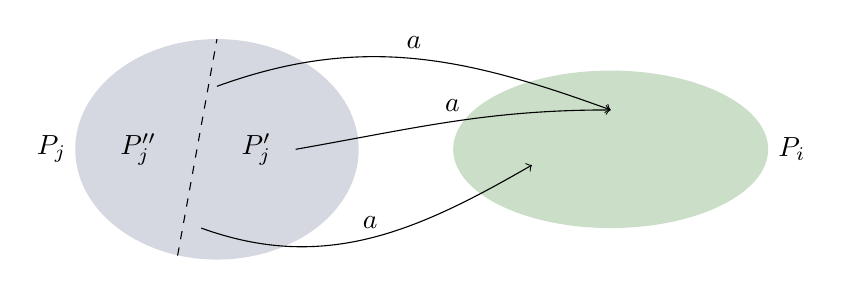
\begin{tikzpicture}
            \definecolor{color1}{RGB}{213, 216, 224}
            \definecolor{color2}{RGB}{202, 222, 200}
            
            \fill[color=color1] (0,0) ellipse (1.8cm and 1.4cm);
            \draw[dashed] (-0.5,-1.35) -- (0,1.4);
            \fill[color=color2] (5,0) ellipse (2cm and 1cm);
            
            \node at (-2.1,0) {$P_j$};
            \node at (-1,0) {$P''_j$};
            \node at (0.5,0) {$P'_j$};
            \node at (7.3,0) {$P_i$};

            \draw[->] (0, 0.8) to[in=160, out=20] node[above]{$a$} (5,0.5);
            \draw[->] (1,0) to[in=180, out=10] node[above]{$a$} (5,0.5);
            \draw[->] (-.2,-1) to[in=210, out=-20] node[above]{$a$} (4,-.2);
        \end{tikzpicture}
    \end{center}
    This set of states can be expressed via the inverse transition function:
    $$ \{q \in P_j\ |\ \delta(q,a) \in P_i \} = \left( \bigcup_{q' \in P_i} \delta^{-1}(q', a)\right) \cap P_j $$
    Since $\delta^{-1}$ was already computed in the first step of the algorithm, we can determine using req.\ \ref{req:3} whether a state of $\bigcup_{q \in P_i} \delta^{-1}(q, a)$ is also in $P_j$ in $\Theta(1)$ time.
    
    Thus, instead of examining $P_j$ for all $j < k$, we rather go through the table of $\delta^{-1}$ and for each state $q$ such that $\delta(q, a) \in P_i$, we know from req.\ \ref{req:4} that we can determine the index $j < k$ (because there are $k$ blocks) of the block $P_j$ containing $q$ in $\Theta(1)$ time. The sets $P'_j$ and $P''_j = P_k$ resulting from the partition can be constructed on the fly without any additional time cost. The construction of the sets $s_{b, j}$ and $s_{b, k}$ as well as the update of $L_b$ for all $b \in \Sigma$ can also be done on the fly but require $\Theta(1)$ time for each symbol $b \in \Sigma$ and thus add up to a total of $\Theta(\left| \Sigma \right|)$ time.
    \ednote{VT}{the on-the-fly computation part is a little hand-waving...}

    Overall, one iteration of the loop runs in time
    $$\Theta \left( \left| \Sigma \right| \cdot \left| \bigcup_{q \in P_i} \delta^{-1}(q, a) \right| \right) $$

    \bigskip
    We now show the result for Algorithm \ref{alg:modern}. A splitter ${s =: (a, C)}$ is picked from $\mathcal{W}$. Then, we iterate over all blocks $B \in \mathcal{P}$ that may be split with $s$. Let $B \in \mathcal{P}$.
    \begin{align*}
        s\ \text{splits}\ B &\iff \exists q_1, q_2 \in B, \delta(q_1, a) \in C \land \delta(q_2, a) \notin C\\
        &\iff \left(\bigcup_{q \in C} \delta^{-1}(q, a)\right)\cap B \neq \varnothing \land \left(\bigcup_{q \in B}\delta(q, a)\right)\setminus C \neq \varnothing
    \end{align*}
    \ednote{VT}{we may express the right-hand conjunct in terms of $\delta^{-1}$ in order to prepare the paragraph that follows (But it wouldn't be the same union because you have to start from states outside $C$)}
    \ednote{VT}{The second equation may be a little too quick, especially for the right-hand conjunct.}
    Likewise, instead of examining all blocks $B \in \mathcal{P}$, we go through $\delta^{-1}$ and we update the splitters for all symbols in $\Sigma$ and one iteration of the loop runs in time
    $$\Theta \left( \left| \Sigma \right| \cdot \left| \bigcup_{q \in C} \delta^{-1}(q, a) \right| \right) $$
\end{proof}

For the sake of simplicity, we now denote $\displaystyle{\bigcup_{q \in C} \delta^{-1}(q, a)}$ by $\overset{\hookleftarrow}{C}$.

We will now justify the logarithmic factor in the time complexity. We briefly explain why a logarithm stands out and prove the statement by induction. The idea is that for each symbol $a \in \Sigma$, a state $q \in \mathcal{Q}$ can be in at most one of the splitters in $\mathcal{W}$. When the loop iterates over this splitter, it will split the block and keep the smaller one, whose size will be at most the size of the splitter divided by two. This means that a splitter $s$ can be processed at most $\log \| s \|$ times. We now properly state and prove the property by induction.

We see splitters as updatable program variables. This means that $s_{a,i}$ as a set may differ along the loop, however we know there exists some $q \in \mathcal{Q}$ such that $s_{a,i}$ is the unique set containing $q$ throughout the execution. This gives a way to characterize splitters throughout the whole execution.

\bigskip

\begin{lemma}\label{lem:log}
    Any splitter in the workset $s \in \mathcal{W}$ is processed -- i.e.\ picked at the beginning of the \textit{while} loop -- at most $\lfloor \log \| s \| \rfloor$ times.
\end{lemma}
\begin{proof}
    We first show the following statement:

    \textit{During an iteration, the chosen splitter $s$ will either be removed from the set of splitters or its size will be reduced by at least $\frac{\| s\|}{2}$ after the iteration\footnote{That is a bit informal because, the original splitter is actually removed and another ``similar'' splitter (cf the paragraph above the statement of the lemma) of size at most $\frac{||s||}{2}$ will be added.}.}

    \bigskip
    Let $\{P_1, \cdots, P_\ell\}$ be the current partition and let $s =: (a, C)$ be the picked splitter. Thus, $s$ is no longer in the set of splitters $\mathcal{W}$. Since we go over all splittable blocks, $C$ may also be split by $s$.
    \begin{itemize}
        \item If $C$ is not split by $s$, then $s$ was already removed from the splitters. Note that it can be added again later if it is split by another splitter.
        \item If $C$ is split into $C'$ and $C''$, then $(a, \min\{C', C''\})$ is added to the splitters and its size is at most $\frac{\| s \|}{2}$.
    \end{itemize}
    Therefore, since a splitter cannot be empty, $s$ can be processed at most $m$ times where $m$ is such that
    $$ 1 \leq \frac{\| s \|}{2^m} < 2$$
    which is equivalent to
    $$ m \leq \log \| s \| < m + 1 \quad \text{i.e.}\quad \left\lfloor\log \| s \|\right\rfloor = m $$
\end{proof}

\bigskip

\begin{lemma}\label{lem:log_non_splitter}
    Any block $B$ resulting from a split and not added as a splitter is processed at most $\lfloor \log \frac{| B |}{2} \rfloor$ times.
\end{lemma}
\begin{proof}
    Let $P \in \mathcal{P}$ be a block in the partition and $s =: (a, C)$ be a splitter such that $s$ splits $P$ into $S$ and $B$ so that $(a, S)$ is added to the workset and $B$ is not. In order for $B$ to be processed, some $(b, B)$ must be added to the workset.
    
    Since the only way to create a fresh splitter is to split $B$, this means that there exists some later step in the loop such that some splitter $(b, B')$ splits $B$ into $B_1$ and $B_2$ and $(b, \min\{B_1, B_2\})$ is added to the workset.

    From lemma \ref{lem:log}, we know that this splitter can be processed at most $\lfloor\log |\min \{B_1,B_2\}|\rfloor$ times. Since $|\min\{B_1, B_2\}| \leq \frac{| B |}{2}$ and since there is no splitter containing $B$ in the workset, we obtain that $B$ can be processed at most $\lfloor\log \frac{| B |}{2}\rfloor$ times.
\end{proof}

\bigskip

\begin{lemma}\label{lem:bound}
    Let us consider some step in the algorithm such that $\mathcal{P}$ is the current partition. The total time spent in the loop until termination is bounded by
    $$ T := \theta \left(\sum_{(a, C) \in \mathcal{W}} | \overset{\hookleftarrow}{C} | \log | C | + \sum_{(a, B) \in (\Sigma\times \mathcal{P})\setminus \mathcal{W}} | \overset{\hookleftarrow}{B} | \log \frac{| B |}{2} \right)$$
    where $\theta$ is the constant of proportionality that may be obtained from lemma \ref{lem:time_iteration}.
\end{lemma}
\begin{proof}
    We show the result by induction over the steps.

    \bigskip
    \textbf{Base case:} the current partition is $\{P_1, P_2\}$ and we may assume w.l.o.g.\ that $P_1$ is the smaller set, so that $\mathcal{W} = \{(a, P_1), a \in \Sigma\}$.
    We have to show that the total time spent in the loop is bounded by
    $$T = \theta |\Sigma| \left(| \overset{\hookleftarrow}{P_1} | \log | P_1 | + | \overset{\hookleftarrow}{P_2} | \log \frac{| P_2 |}{2}\right)$$
    
    We know from lemma \ref{lem:time_iteration} that an iteration of the loop for $(a, P_i)$ takes $\theta | \overset{\hookleftarrow}{P_i} | $ time.
    \begin{itemize}
        \item From lemma \ref{lem:log}, for all $a\in\Sigma$, $(a, P_1)$ can be processed at most $\log \| (a, P_1) \| = \log |P_1|$ times\footnote{We drop the floor operator for simplicity. Note that since we are giving upper bounds, this is completely valid.}, hence the total time for $(a, P_1)$ is bounded by $\theta | \overset{\hookleftarrow}{P_1} | \log | P_1 |$ and thus the total time for splitters with block $P_1$ is bounded by
        $$\theta |\Sigma| | \overset{\hookleftarrow}{P_1} | \log | P_1 |$$

        \item From lemma \ref{lem:log_non_splitter}, for all $a\in\Sigma$, $(a, P_2)$ can be processed at most $\log \frac{\| (a, P_2) \|}{2} = \log \frac{| P_2 |}{2}$ times. Thus, the total time for non splitters with block $P_2$ is bounded by
        $$ \theta |\Sigma| | \overset{\hookleftarrow}{P_2} | \log \frac{| P_2 |}{2}$$
    \end{itemize}
    
    \textbf{Inductive step:} Let $\{P_1, \cdots, P_\ell\} := \mathcal{P}$ be the current partition. The induction hypothesis states that the total time spent in the loop until termination for $a$ is bounded by
    $$ T := \theta \left(\sum_{(a, C) \in \mathcal{W}} | \overset{\hookleftarrow}{C} | \log | C | + \sum_{(a, B) \in \Sigma\times \mathcal{P}\setminus \mathcal{W}} | \overset{\hookleftarrow}{B} | \log \frac{| B |}{2} \right)$$
    By going through one more step, some blocks of $\mathcal{P}$ may be split and we define a new time $\hat{T}$ over this new partition and we have to show that $\hat{T} \leq T$.

    Suppose some $B \in \mathcal{P}$ is split into $B'$ and $B''$ by any splitter.
    We have to consider the cases where $(a , B)$ is a splitter or not for all $a \in \Sigma$. Let $a \in \Sigma$.
    \begin{itemize}
        \item $(a, B) \in \mathcal{W}$: $\mathcal{W}$ is updated as follows:
        $$ \mathcal{W} := \mathcal{W} \setminus \{(a, B)\} \cup \{(a, B'), (a, B'')\}$$
        Thus, instead of taking a time $\theta | \overset{\hookleftarrow}{B} | \log | B |$ time for $(a, B)$, it now takes a time bounded by:
        $$\theta | \overset{\hookleftarrow}{B'} | \log | B' | + \theta | \overset{\hookleftarrow}{B''} | \log | B'' |$$
        Finally, we show the following:
        \begin{equation*}
            | \overset{\hookleftarrow}{B'} | \log | B' | + | \overset{\hookleftarrow}{B''} | \log | B'' | \leq | \overset{\hookleftarrow}{B} | \log | B |
        \end{equation*}
        From $B = B' \cup B''$, we get $|B| = |B'| + |B''|$ and $| \overset{\hookleftarrow}{B} | = | \overset{\hookleftarrow}{B'} | + | \overset{\hookleftarrow}{B''} |$, hence:
        \begin{align*}
            & |\overset{\hookleftarrow}{B'} | \log | B' | + | \overset{\hookleftarrow}{B''} | \log | B'' | - | \overset{\hookleftarrow}{B} | \log | B | \\
            &= | \overset{\hookleftarrow}{B'} | \log | B' | + (| \overset{\hookleftarrow}{B} | - | \overset{\hookleftarrow}{B'}|) \log \left(|B|-|B'|\right) - | \overset{\hookleftarrow}{B} | \log | B | \\
            &= | \overset{\hookleftarrow}{B'} | \log \frac{|B'|}{|B|-|B'|} + | \overset{\hookleftarrow}{B} | \log \frac{|B|-|B'|}{|B|} \\
            &\leq | \overset{\hookleftarrow}{B'} | \log \frac{|B|}{|B|-|B'|} + | \overset{\hookleftarrow}{B} | \log \frac{|B|-|B'|}{|B|} \\
            &= (| \overset{\hookleftarrow}{B}| - |\overset{\hookleftarrow}{B'} |) \log \underset{\leq 1}{\underbrace{\frac{|B|-|B'|}{|B|}}} \leq 0
        \end{align*}

        \item $(a, B) \notin \mathcal{W}$: $(a, \min\{B', B''\})$ is added to the set of splitters. We may assume w.l.o.g.\ that $B'$ is the smaller set. Thus, the corresponding term in the sum $|\overset{\hookleftarrow}{B}| \log \frac{| B |}{2}$ is updated as follows:
        \begin{equation*}
            \theta | \underset{\text{lemma \ref{lem:log}}}{\underbrace{\overset{\hookleftarrow}{B'} | \log | B' |}} + \theta \underset{\text{lemma \ref{lem:log_non_splitter}}}{\underbrace{|\overset{\hookleftarrow}{B''} | \log \left(\frac{| B'' |}{2}\right)}}
        \end{equation*}
        Since $B = B' \cup B''$, the sum above can be written as:
        \begin{equation*}
            \theta | \overset{\hookleftarrow}{B'} | \log | B' | + \theta (| \overset{\hookleftarrow}{B} | - | \overset{\hookleftarrow}{B'} |) \log \left(\frac{|B|-|B'|}{2}\right)
        \end{equation*}
        By using the fact that $\displaystyle{| B' | \leq \frac{|B|}{2}}$, we have:
        \begin{align*}
            & | \overset{\hookleftarrow}{B'} | \log | B'| + (| \overset{\hookleftarrow}{B} | - | \overset{\hookleftarrow}{B'}|)\log \left(\frac{| B | - |B'|}{2} \right) - |\overset{\hookleftarrow}{B}| \log \frac{|B|}{2} \\
            & \leq | \overset{\hookleftarrow}{B'}| \log \frac{| B |}{2} + (| \overset{\hookleftarrow}{B}| - | \overset{\hookleftarrow}{B'}|) \log \left(\frac{|B| - |B'|}{2}\right) - | \overset{\hookleftarrow}{B}| \log \frac{| B |}{2} \\
            & \leq (| \overset{\hookleftarrow}{B}| - | \overset{\hookleftarrow}{B'} |) \log \left(\frac{| B | - | B' |}{| B |}\right) \leq 0
        \end{align*}

        Overall, splitting any block of $\mathcal{P}$ does not increase the total time spent over the loop. By iterating over all blocks, we obtain that the total time $\hat{T}$ spent in the loop from this new iteration until termination is such that $\hat{T} \leq T$.
    \end{itemize}
\end{proof}

\bigskip

\begin{theorem}
    \label{thm:complexity}
    Algorithm \ref{alg:original} runs in $O\left(|\Sigma|\cdot|\mathcal{Q}| \log |\mathcal{Q}|\right)$ time.
\end{theorem}
\begin{proof}
From lemma \ref{lem:bound}, we obtain in particular that for the initial partition the time spent in the loop until termination is bounded by:
$$T = \theta |\Sigma| \left(| \overset{\hookleftarrow}{P_1} | \log | P_1 | + | \overset{\hookleftarrow}{P_2} | \log \frac{| P_2 |}{2}\right)$$
Thus, the following holds:
$$T \leq \theta |\Sigma| (\underset{\leq 2|\overset{\hookleftarrow}{\mathcal{Q}}|}{\underbrace{|\overset{\hookleftarrow}{P_1}| + |\overset{\hookleftarrow}{P_2}|}})\log(\underset{= |\mathcal{Q}|}{\underbrace{|P_1| + |P_2|}}) \leq 2 \theta|\Sigma||\mathcal{Q}| \log |\mathcal{Q}|$$
\end{proof}

% \printglossary[type=\acronymtype]

% \addcontentsline{toc}{section}{CV}
% \includepdf{cv.pdf}

\pagebreak
% bibliography
\bibliographystyle{alpha}
\bibliography{ref}

\end{document}